\documentclass[]{article}
\usepackage{lmodern}
\usepackage{amssymb,amsmath}
\usepackage{ifxetex,ifluatex}
\usepackage{fixltx2e} % provides \textsubscript
\ifnum 0\ifxetex 1\fi\ifluatex 1\fi=0 % if pdftex
  \usepackage[T1]{fontenc}
  \usepackage[utf8]{inputenc}
\else % if luatex or xelatex
  \ifxetex
    \usepackage{mathspec}
  \else
    \usepackage{fontspec}
  \fi
  \defaultfontfeatures{Ligatures=TeX,Scale=MatchLowercase}
\fi
% use upquote if available, for straight quotes in verbatim environments
\IfFileExists{upquote.sty}{\usepackage{upquote}}{}
% use microtype if available
\IfFileExists{microtype.sty}{%
\usepackage{microtype}
\UseMicrotypeSet[protrusion]{basicmath} % disable protrusion for tt fonts
}{}
\usepackage[margin=1in]{geometry}
\usepackage{hyperref}
\hypersetup{unicode=true,
            pdfborder={0 0 0},
            breaklinks=true}
\urlstyle{same}  % don't use monospace font for urls
\usepackage{graphicx,grffile}
\makeatletter
\def\maxwidth{\ifdim\Gin@nat@width>\linewidth\linewidth\else\Gin@nat@width\fi}
\def\maxheight{\ifdim\Gin@nat@height>\textheight\textheight\else\Gin@nat@height\fi}
\makeatother
% Scale images if necessary, so that they will not overflow the page
% margins by default, and it is still possible to overwrite the defaults
% using explicit options in \includegraphics[width, height, ...]{}
\setkeys{Gin}{width=\maxwidth,height=\maxheight,keepaspectratio}
\IfFileExists{parskip.sty}{%
\usepackage{parskip}
}{% else
\setlength{\parindent}{0pt}
\setlength{\parskip}{6pt plus 2pt minus 1pt}
}
\setlength{\emergencystretch}{3em}  % prevent overfull lines
\providecommand{\tightlist}{%
  \setlength{\itemsep}{0pt}\setlength{\parskip}{0pt}}
\setcounter{secnumdepth}{0}
% Redefines (sub)paragraphs to behave more like sections
\ifx\paragraph\undefined\else
\let\oldparagraph\paragraph
\renewcommand{\paragraph}[1]{\oldparagraph{#1}\mbox{}}
\fi
\ifx\subparagraph\undefined\else
\let\oldsubparagraph\subparagraph
\renewcommand{\subparagraph}[1]{\oldsubparagraph{#1}\mbox{}}
\fi

%%% Use protect on footnotes to avoid problems with footnotes in titles
\let\rmarkdownfootnote\footnote%
\def\footnote{\protect\rmarkdownfootnote}

%%% Change title format to be more compact
\usepackage{titling}

% Create subtitle command for use in maketitle
\providecommand{\subtitle}[1]{
  \posttitle{
    \begin{center}\large#1\end{center}
    }
}

\setlength{\droptitle}{-2em}

  \title{}
    \pretitle{\vspace{\droptitle}}
  \posttitle{}
    \author{}
    \preauthor{}\postauthor{}
    \date{}
    \predate{}\postdate{}
  

\begin{document}

\hypertarget{the-punch-line-first}{%
\section{The Punch Line First}\label{the-punch-line-first}}

For this workshop we are starting at the end and working backwards. As
such this first lesson is going to be in a follow the leader mode. This
is a useful way to teach this as we get to see what is possible early on
and then we can focus on the details of how we get there and you will
have a working example of an R script that includes a full data
analysis. Let's get started:

\hypertarget{create-a-new-project-in-rstudio}{%
\subsection{Create a new project in
RStudio}\label{create-a-new-project-in-rstudio}}

We will use the RStudio ``\url{File:New} Project'' dialog to create a
new project to house our work for this workhsop. In RStudio you need to
find the New Project menu.

\begin{figure}
\centering
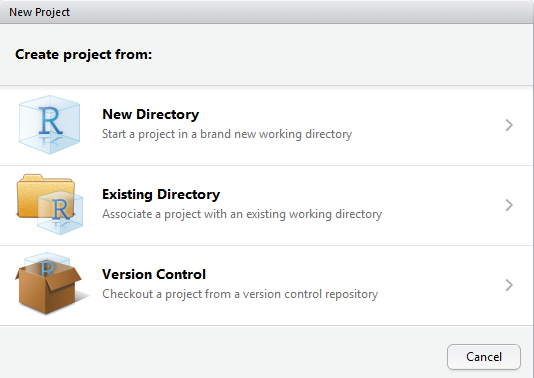
\includegraphics{figures/rstudio_proj1.png}
\caption{rstudio\_proj1}
\end{figure}

Then select ``New Diectory''

\begin{figure}
\centering
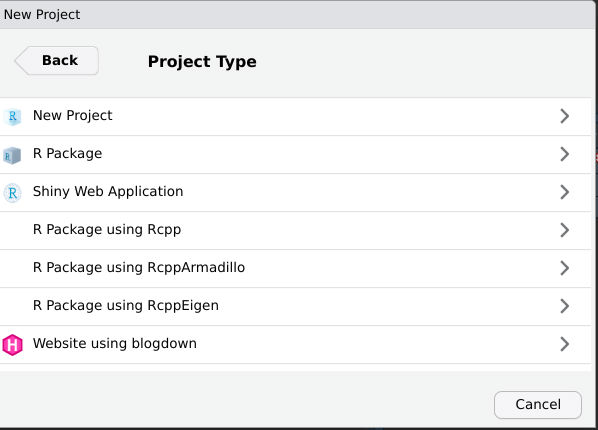
\includegraphics{figures/rstudio_project_new.jpg}
\caption{new directory}
\end{figure}

Then select ``New Project''

\begin{figure}
\centering
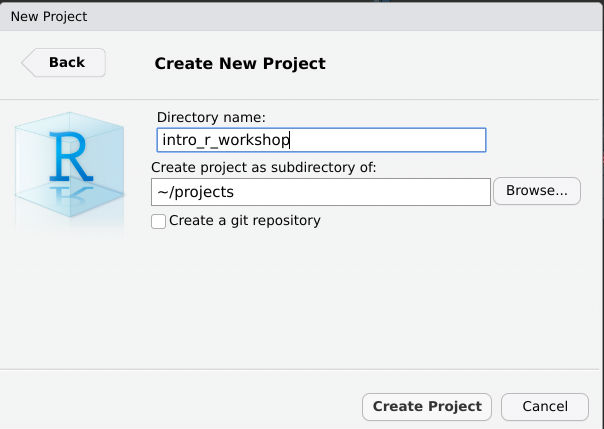
\includegraphics{figures/rstudio_project_new2.jpg}
\caption{rstudio\_proj1}
\end{figure}

The select ``Create Project.'' Name this project ``usepa\_intro\_r''. At
this point you should now have a new, empty project. We need to download
the R Script and some data that we will be using for our workshop. Right
click on each of the the links below and select ``Save Link As''. In the
window that opens up, browse to the location of the project and save
these files to the project folder. Chrome seems to want to call the data
file, a ``.txt'' file. It shouldn't do that, but it does. Make sure that
you change the ``.txt'' to ``.csv'' when you save the file.

\begin{itemize}
\tightlist
\item
  \href{https://raw.githubusercontent.com/usepa/intro_r_workshop/master/lessons/nla_analysis.R}{NLA
  R Analysis}
\item
  \href{https://www.epa.gov/sites/production/files/2014-10/nla2007_chemical_conditionestimates_20091123.csv}{2007
  NLA Water Quality Data}
\end{itemize}

\hypertarget{run-the-script}{%
\subsection{Run the script}\label{run-the-script}}

And now we can run the script by selecting all lines
(i.e.~\texttt{ctrl-a}) and then clicking on the \texttt{Run} button

\begin{figure}
\centering
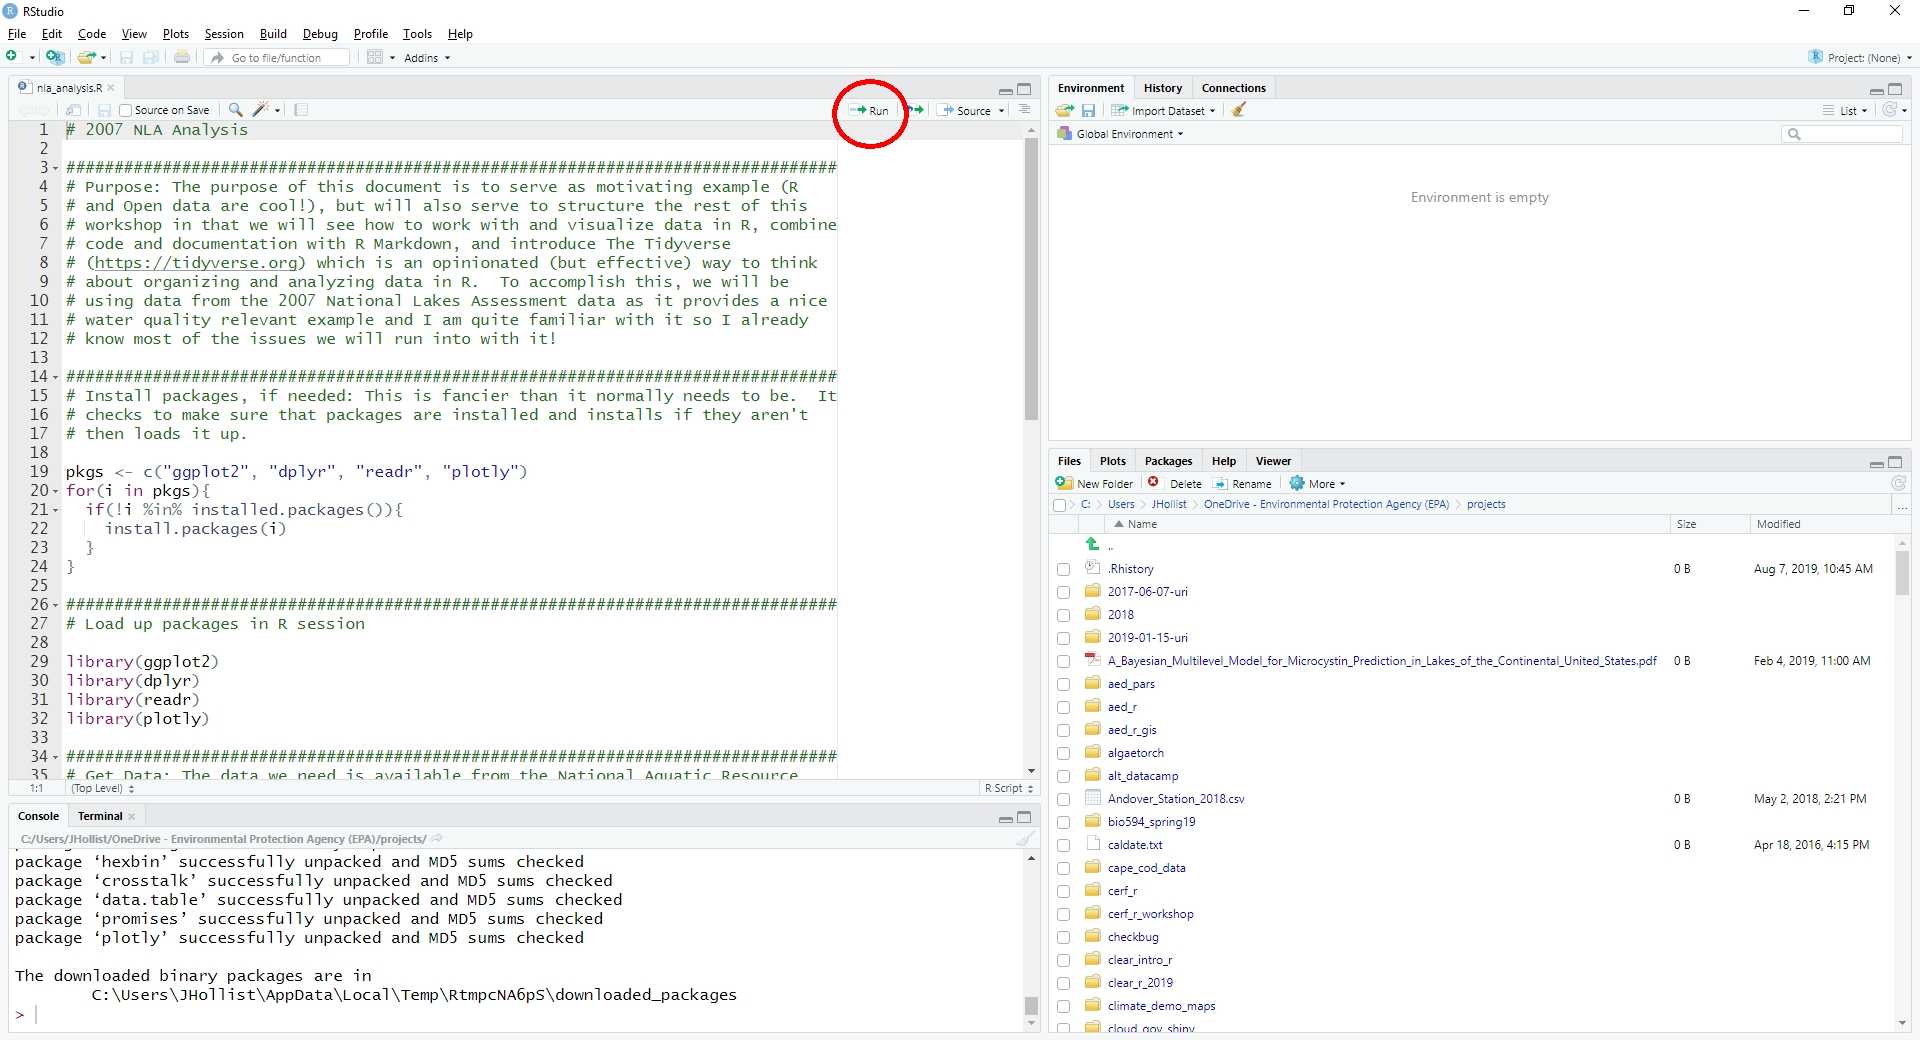
\includegraphics{figures/rstudio_run.jpg}
\caption{rstudio\_knit}
\end{figure}


\end{document}
